\documentclass[tikz,border=2mm]{standalone}
\usetikzlibrary{calc,quotes,intersections, angles}
\usepackage{tkz-euclide} %for right angle marker

\begin{document}
    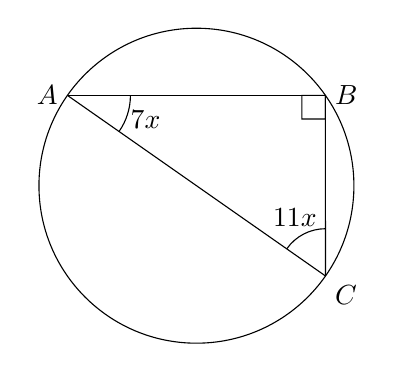
\begin{tikzpicture}[scale=2]
    %mark points on circle
        \coordinate[label=right:$B$] (B) at (35:1);
        \coordinate[label=left:$A$] (A) at (145:1);

    %draw chords and circle
        \draw[name path=circ] (0,0) circle (1);
        \draw (B) -- (A);
  
    \path[name path=BC] (B) -- ($(B)!1!90:(A)$);
    \path[name intersections={of=BC and circ, by={temp,C}}];
          
    \draw (B) -- (C);
    \draw (A) -- (C);
    \node at (C) [anchor = north west] {$C$};
    
        \pic [draw, "$7x$", angle eccentricity=1.3, angle radius = 0.8cm] {angle = C--A--B};
        \pic [draw, "$11x$", angle eccentricity=1.4, angle radius = 0.6cm] {angle = B--C--A};

    %marking right angles
    \tkzMarkRightAngle[size=.15](A,B,C);
        
    \end{tikzpicture}
\end{document}